\chapter{Development Process}
We decided to use an adaptation of the agile method Scrum for the project, due to the uncertainties we faced with handling hardware for the first time. The project requires us to understand the hardware, how the radio frequency modules transmits and receives data amongst them. This meant that using a plan driven method would be hard as planning the whole project would be a difficult task, since we cannot be certain that we have understood the requirements of the project correctly.
However in the initial stage of requirements engineering, a somewhat spiral model of the development process is used. The spiral model can be seen on \myref{fig:spiralDiagram}.

\begin{figure}[ht]
\centering
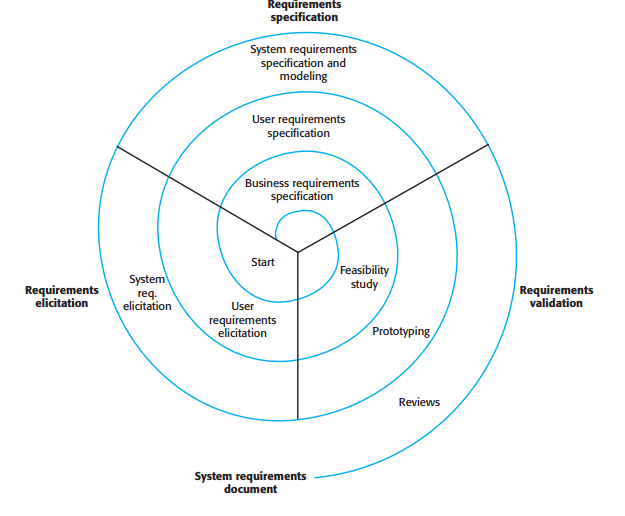
\includegraphics[width=0.80\textwidth]{Figures/spiral.png}
\caption{Spiral Model for requirements engineering \citep[p.112]{SOEBOOK}}\label{fig:spiralDiagram}
\end{figure}

At the start of the project much is not known about the hardware and what requirements this produces for the project, therefore using the spiral method to slowly gain knowledge of the requirements will be a good idea. First getting the knowledge available from external sources about how the hardware can be used and also how powerful it is, and further testing this knowledge by prototyping and testing the communication between devices. 
Once the spiral method has been completed a system requirements document will have been created, and from there an adaptation of Scrum will be used.
We do not have a product owner for the project, which means that this roll for Scrum will go unused. The roll is a big part of the scrum methodology, but we deem that since there is no product owner, it is us in the group who will be explaining the requirements of the project from what we learn in the requirements engineering phase. 

Scrum makes us able to work on the project in an incremental way, and our project is actually easily seperated into increments.
To give a quick example of this, the increments could be: a) establishing a connection between 2 devices, b) establishing a connection with 3 devices, where 2 of the devices cannot reach eachother, and this can continue for a while.
The incrementability of the project calls for an iterative development process, which further arguments for our use of Scrum.
Another reason for us to use Scrum is also for the benefits of continuouslyworking with shorter deadlines in the form of sprints and hopefully the last month of development will not be as stresful as it could have been.